\documentclass{article}
\usepackage{graphicx}
\usepackage[margin=2cm]{geometry}
\usepackage{hyperref}
\usepackage{cite}
\usepackage{subcaption}

\title{\Huge \textbf{AppleStocks}\\\vspace{0.2em} \Large A Simple Application for Apple Stock Quotes Monitoring}
\author{
    Henrique Romão \\ 
    \textit{up202108067@up.pt} 
    \and 
    Mariana Bessa \\ 
    \textit{up202107946@up.pt}
}

\setlength{\parindent}{0em}
\setlength{\parskip}{0.7em}
\setcounter{tocdepth}{2}
\begin{document}

\maketitle

\begin{abstract}
    To be written at the end.
    % [TO-DO]
\end{abstract}

\tableofcontents

\newpage

\section{Introduction}
This application was developed to provide users with a simple and intuitive way to view Apple stock quotes for a selected recent period. 
Users can customize their experience by choosing the time interval, in days or hours, and the duration of the interval, ranging from 2 to 10.

\section{Use Cases}
The application supports the following use cases, which are represented in the use case diagram, in Figure \ref{fig:UseCases}.
\begin{itemize}
    \item Choose View Options - where the user selects a time interval (Hourly or Daily) and a range (2–10).
    \item Get Stock Information - where the application connects with the Web API.
    \item See Stocks - when the user pushes the "Submit" button and sees the Plot Activity.
\end{itemize}

\begin{figure}[ht]
    \centering
    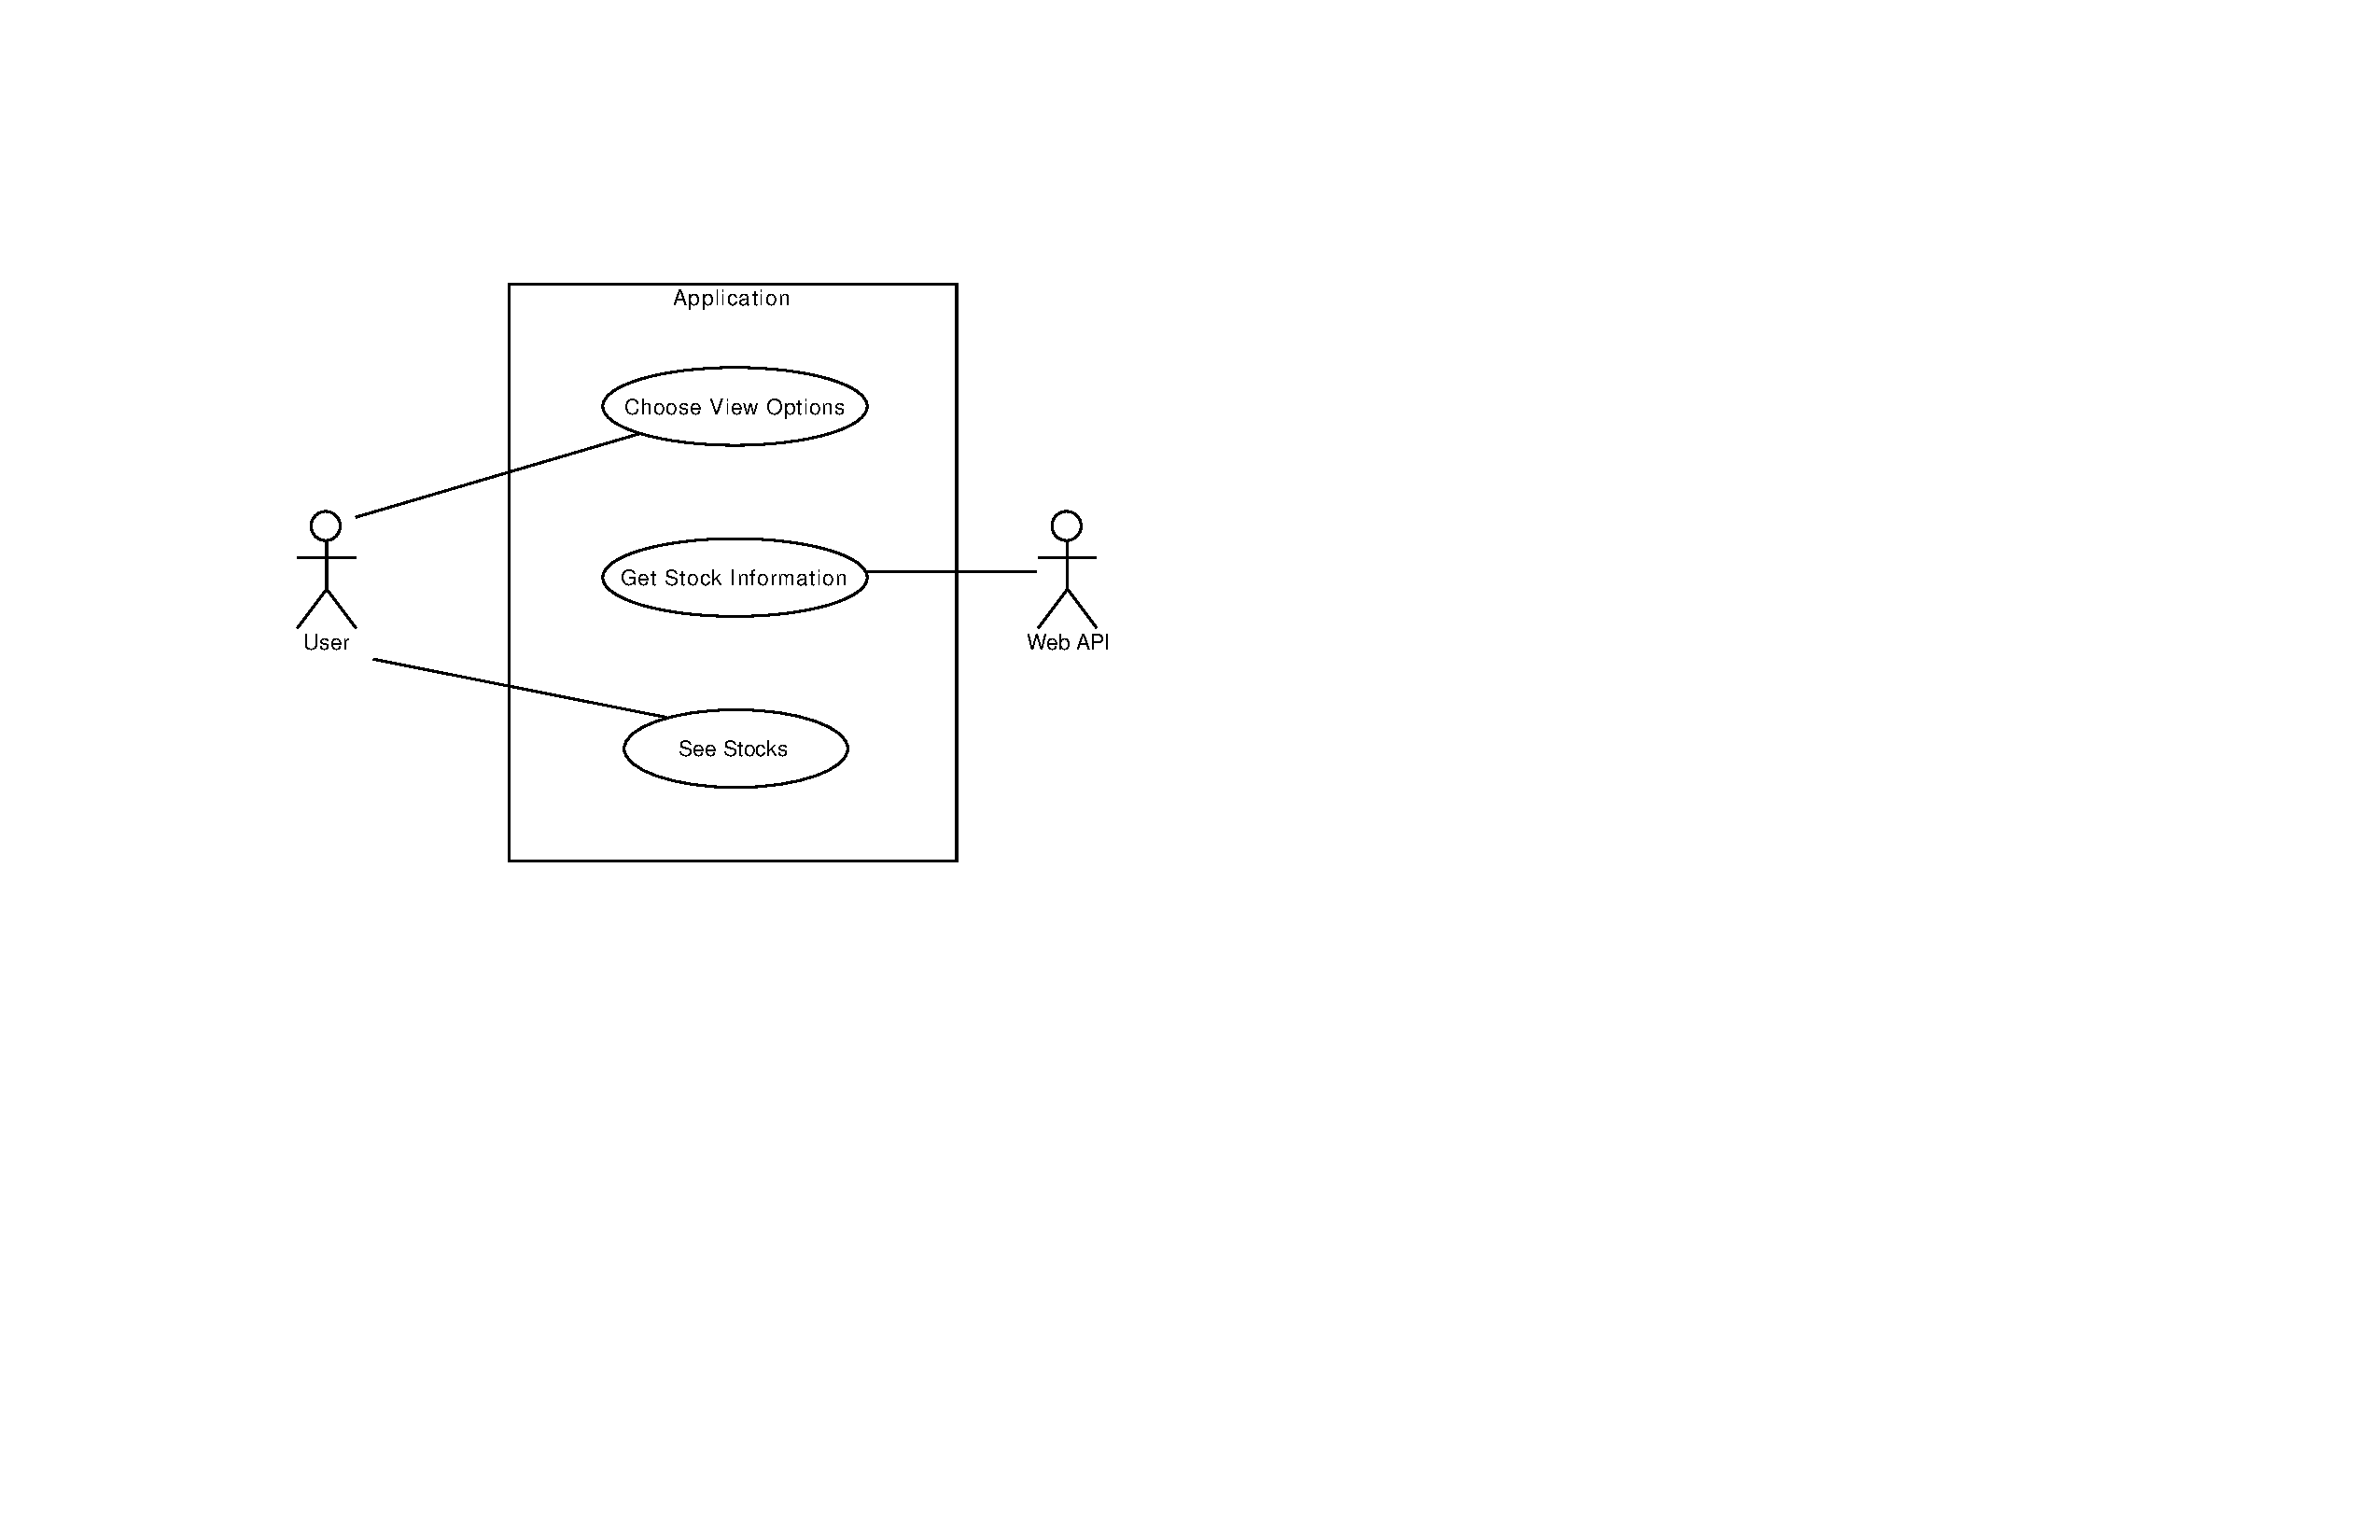
\includegraphics[width=0.6\linewidth]{Use Cases.pdf}
    \caption{Use Cases Diagram.}
    \label{fig:UseCases}
\end{figure}

\section{Architecture}
% This application was developed to offer users a straightforward and intuitive way to view Apple stock quotes over a chosen recent period. Users can adjust their experience by selecting the type of time interval (in days or hours) and the duration of the interval, which can range from 2 to 10 intervals.
% [COMMENT][HR] acho que isto já é um pouco repetitivo que vamos dizer na introdução e abstract

To make the application more user-friendly and less crowded, the application was divided into two activities: the Main Activity, where the user configures their preferences, and the Plot Activity, where the results are displayed.

\subsection{Action Bar}
Common to both activities, there is an action bar displaying the name of the app. 

\subsection{Main Activity}
\label{sec:Main Activity Java}

It also includes two \textbf{Spinner} objects: one for selecting the type of interval (hours or days) and another for specifying the interval range. 
These spinners are initialized in the Main Activity code using the \texttt{new ArrayAdapter<>()} method, with \texttt{setDropDownViewResource} used to define their layout.

Both spinners have default values: "H" (hours) for the type of interval and "2" for the range. 
This means that, unless changed by the user, the stock quotes for the last two hours will be displayed by default.

A button is provided to allow the user to proceed. Its listener is implemented within the Main Activity. The \texttt{onClick()} method creates an \textbf{Intent} to open the Plot Activity, passing the user's spinner selections (as a string and an integer) to the new activity.

\subsection{Plot Activity}
In the plot activity is where, according to the choices made on the Main Activity, the HTTPS request is made, retrieving the stock information from the web API, and where the request is processed, displaying the information to the user.

\subsubsection{HTTP Request}
The first step is to read the intent passed from the previous activity, retrieving the time interval type and total number.
With these two variables, it is possible to craft the URL, which will be used to do the HTTP request.

The URL for the HTTP request, passed through a function that initiates a new thread where the rest of the processing will take place.
Inside the thead, the processing is initiated by the \texttt{FetchData} private class, that takes a URL and establishes the HTTP connection.
The connection status is assessed, and if it is succesfull, the processing will go on, otherwise, an error message is thrown.

\subsubsection{Data Processing}
Before the actual processing begins, the input stream received from the HTTP connection is converted into type \texttt{String}.
With this \texttt{String}, function \texttt{processJsonData} will create a JSON object retrieve the closing quote prices and respective time.
Redarding the time, it is necessary to convert the dates into timestamps, for the plot function, and so it is necessary to format the dates.
A problem that arises is that, according to the choice of days or hours, the date format will be different, as it will include the hour and timezone in the last case.
To deal with the different formats, according to the selected time interval type, passed through the intent, a different format is used for pasing the date strings into date objects, which are then converted to timestamps.

\subsubsection{Data Plotting}
This processed information is then passed to the \texttt{plotData} function.
The data is plotted using the LineData widget, part of the MPandroid Chart library, \cite{MPAndroidChart}.
This widget was choosen to allow for faster app development, taking use of already developed code, and considering its widespread use, it seemed a correct fit for the problem.
For this widget the data is passed in an array of entries, and so the function joing the two arrays into a single array of entries with two values, one entrie for each dot in the plot.
Additionally, the function also computes the maximum and minimum closing quote prices, and creates an entry array for each, to be plotted as horizontal lines delimiting the maximum and minimum value.
Then, each entry array is properly formatted, and sent to the widget to be plotted.
It is also necessary to format the x axis, otherwise the values seen would be the timestamps, which are difficult to interpret and not user-friendly.
This way, the value is formatted to return a simple date string, and only the first and last values are shown, for a simpler graph analysis.
The maximum and minimum values are also shown outside the plot.

\section{Interface}
The application has a black background with purple accents, as these darker colors are more associated with the stock market. The theme used was \texttt{Theme.AppCompat.Light.DarkActionBar}.

\subsection{Main Activity}
Upon opening the application, the user is welcomed by an action bar and two text views that display a greeting and provide instructions on how to use the app. Below these, additional text views explain the purpose of each spinner.

The layout is organized within a \textbf{LinearLayout} to arrange the text views, spinners, and the submit button vertically. The design ensures that the interface adapts well to both vertical and horizontal screen orientations, maintaining a consistent and user-friendly layout.

When the "Submit" button is pressed, the application launches the Plot Activity using the \texttt{startActivity()} method, passing the user's selected options as extras.

The layout of the spinner items and drop-down items was customly made in the \texttt{/layout/spinner\_dropdown\_ item.xml} and \texttt{/layout/spinner\_item.xml} files. 
The values displayed in the Spinner views were defined in the \texttt{strings.xml} file located in \texttt{src/main/res/values/}. The button was adapted to one with rounder corners through the 

% [COMMENT] [BESSA] HENRIQEU HELP ESTA A SAIR DAS MARGENS
% [HR] é só dar espaço em alguns pontos e ele ajeita

\subsection{Plot Activity}
The interface for the plot activity can be seen in Figure \ref{fig:plot activity}, with the activity still loading the data (Figure \ref{fig:loading}) and with all the data loaded (Figure \ref{fig:plot loaded}).
The activity takes a short time loading, but this wait is due to slow connectivity of the web API, having tested the speed for the same request in our personal computers and noticing a slight delay.

\begin{figure}[ht]
    \centering
    
    \begin{subfigure}[t]{0.49\textwidth}
        \centering
        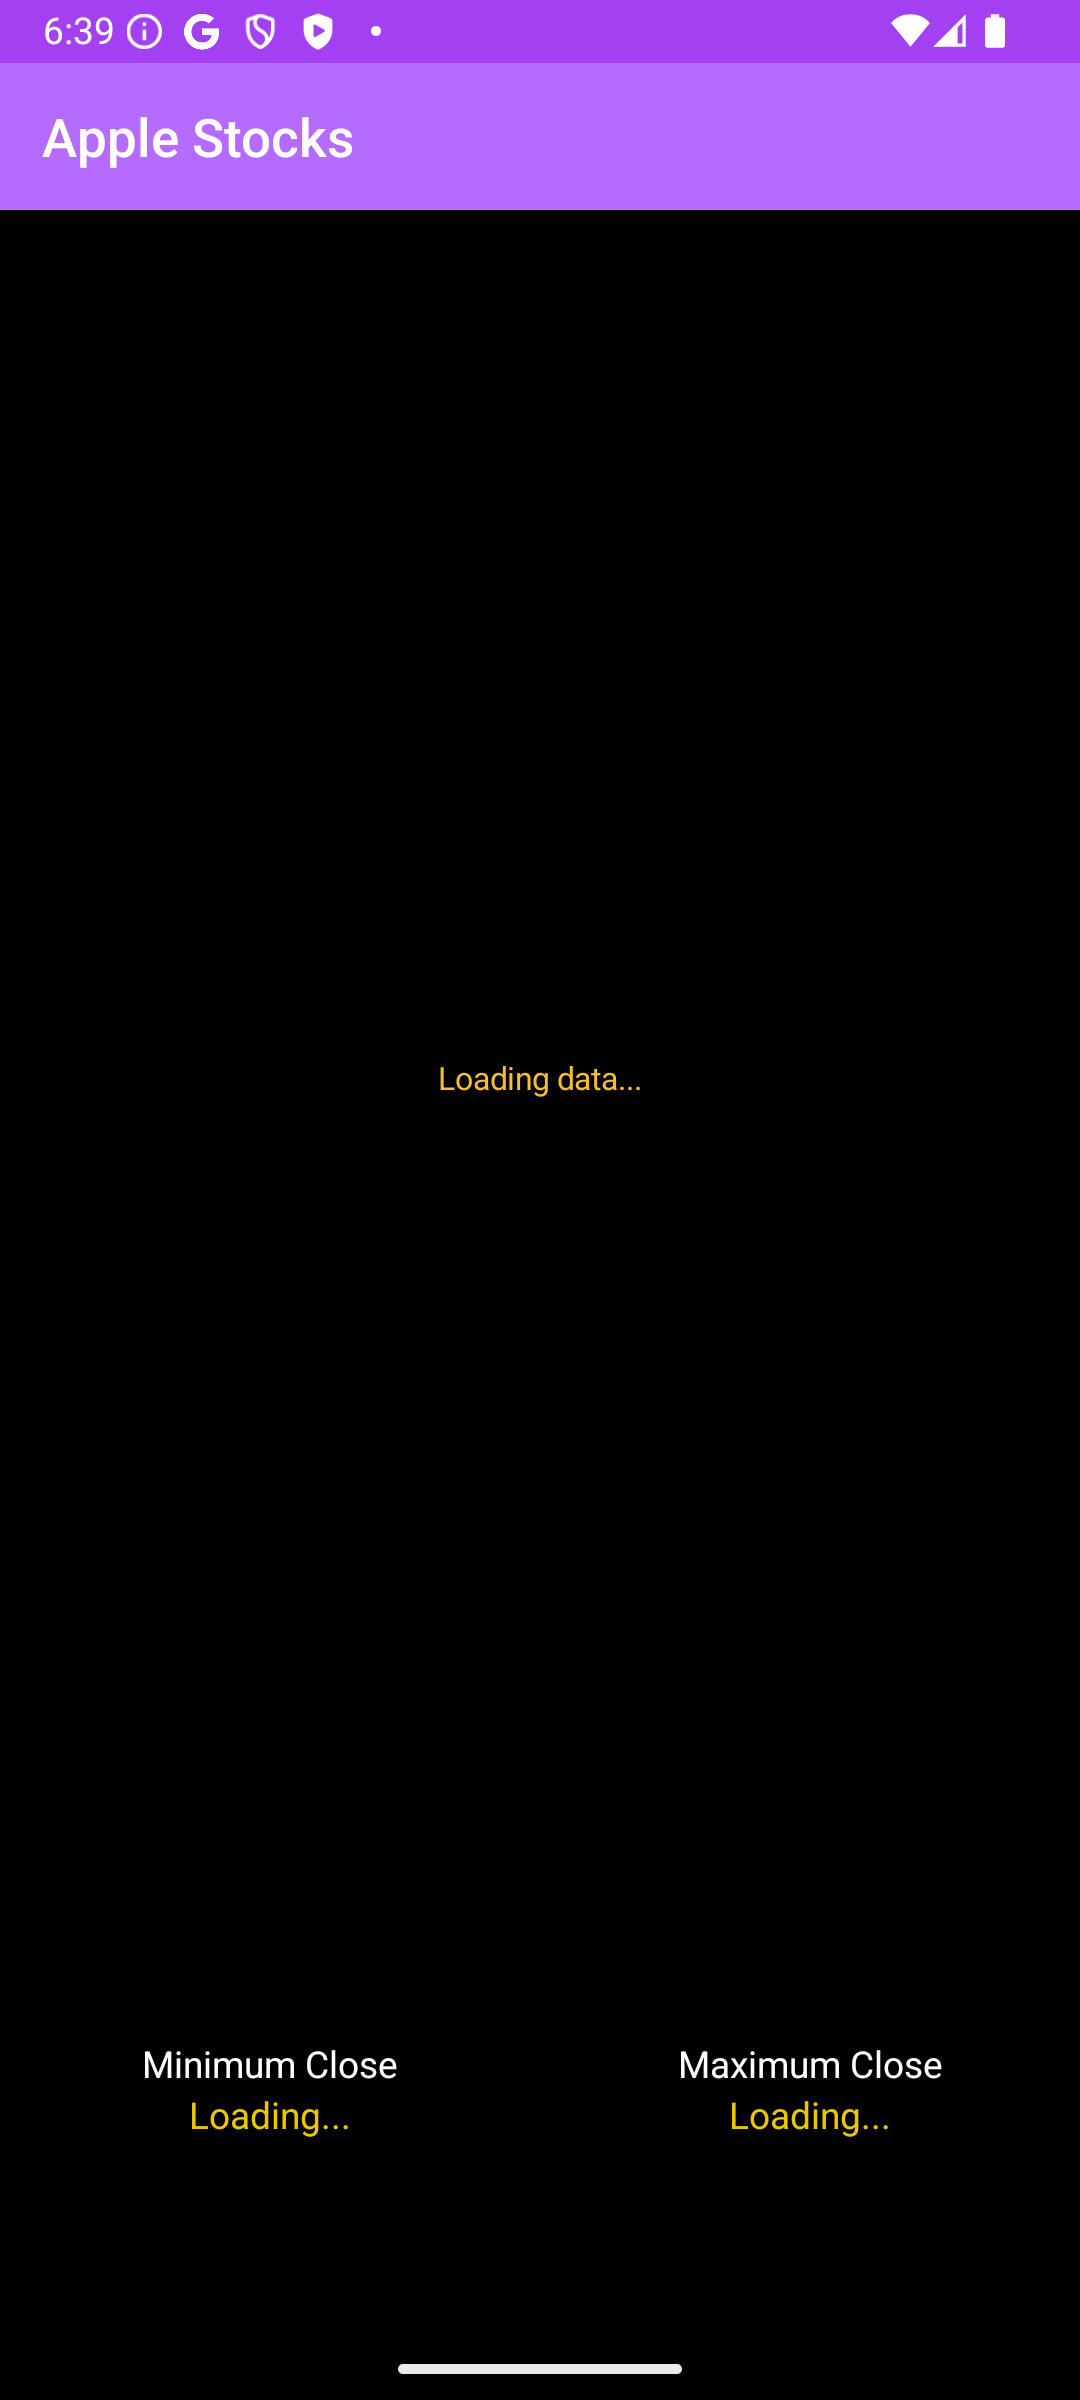
\includegraphics[height=40em]{Imagens/Loading.png}
        \caption{While Loading.}
        \label{fig:loading}
    \end{subfigure}
    \hfill
    \begin{subfigure}[t]{0.49\textwidth}
        \centering
        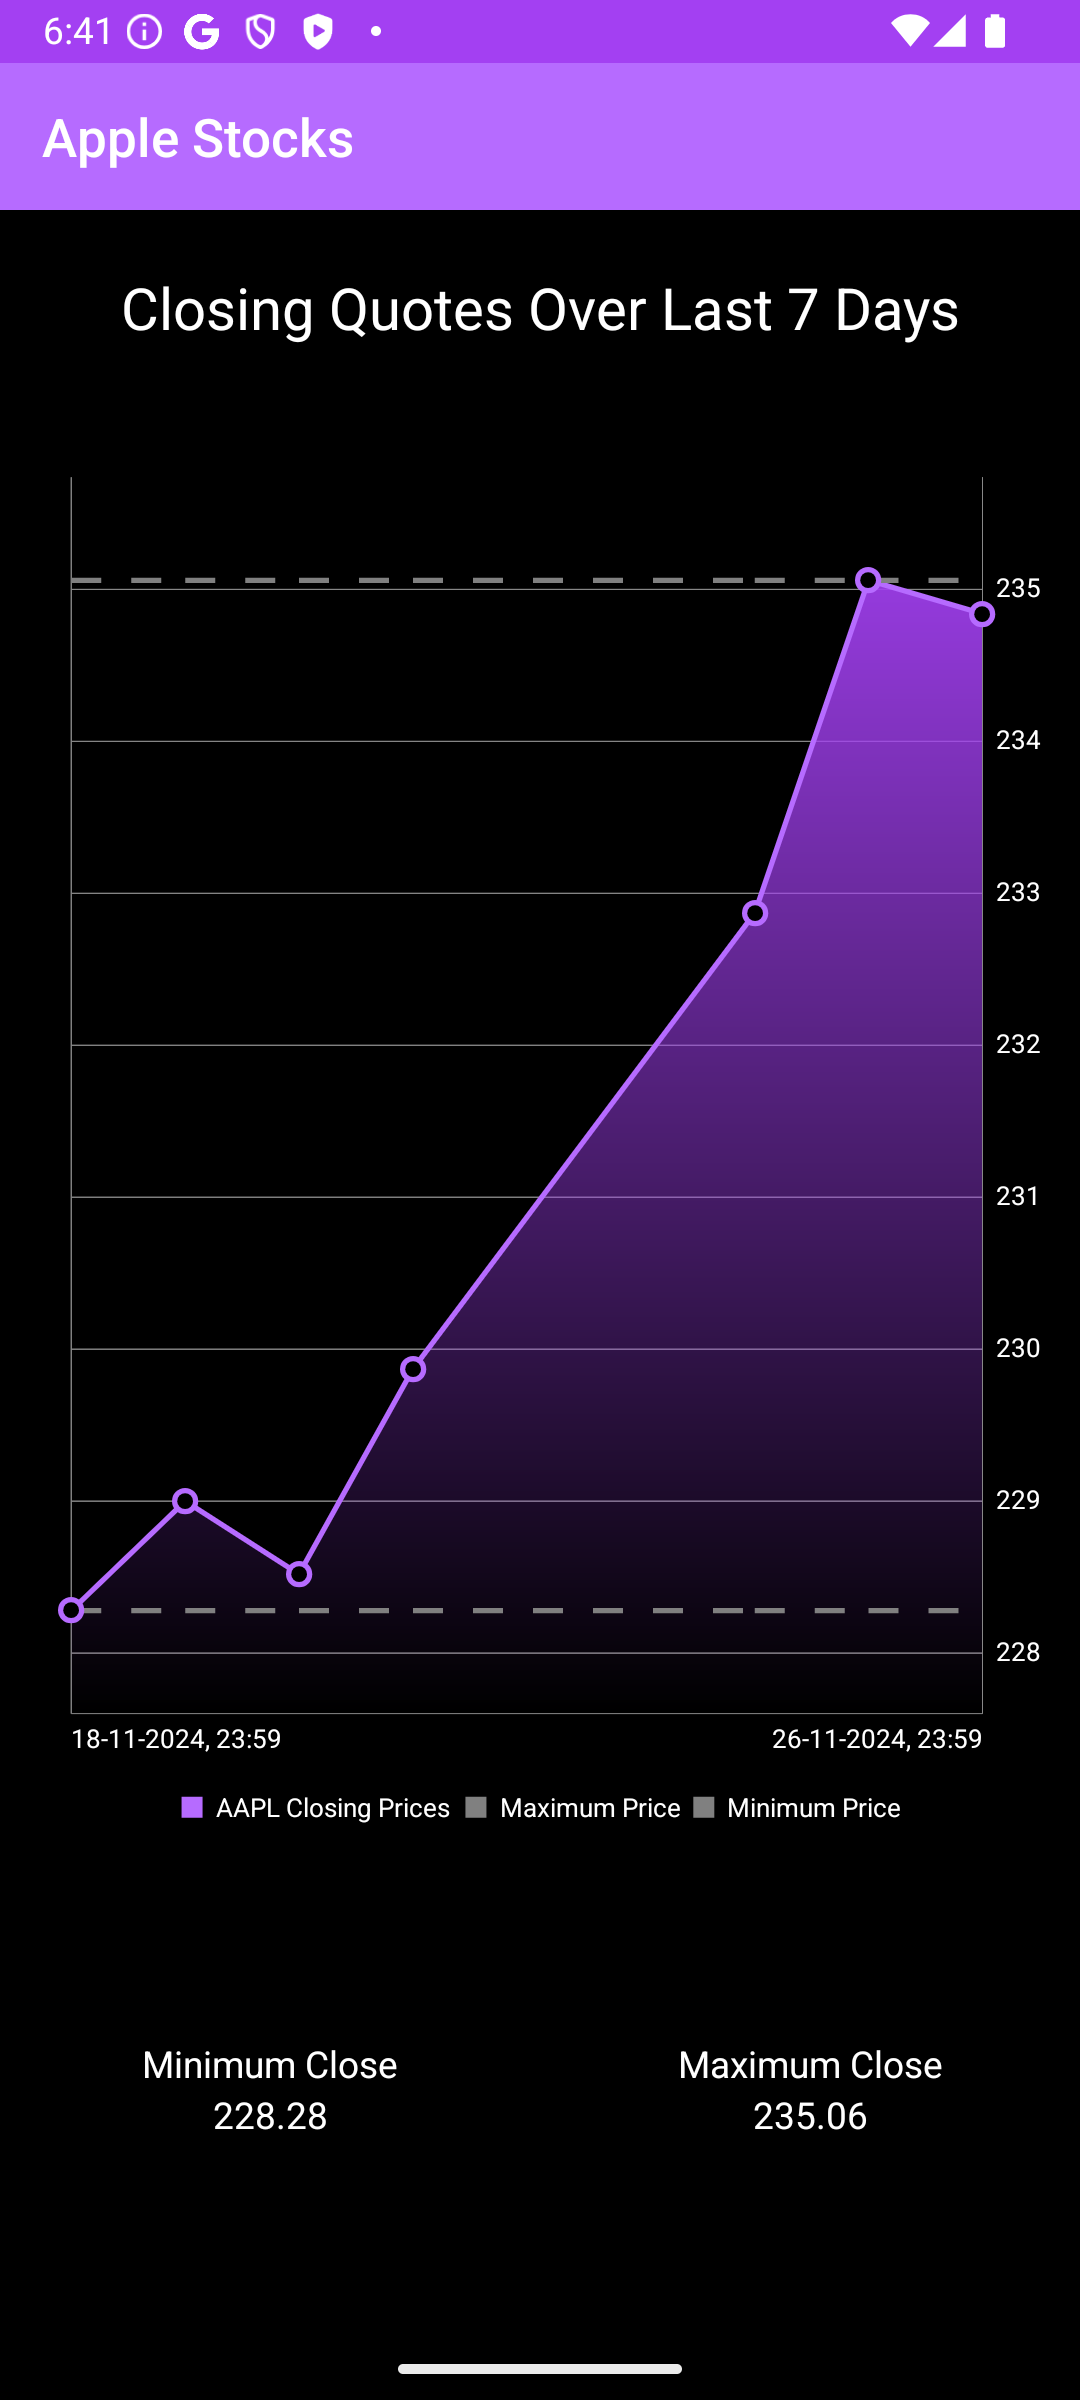
\includegraphics[height=40em]{Imagens/7days.png}
        \caption{Loaded.}
        \label{fig:plot loaded}
    \end{subfigure}

    \caption{Plot Activity.}
    \label{fig:plot activity}
\end{figure}

To have an indication of chosen time intervals, the number of time intervals and time interval type are written in the plot title.

\subsubsection{Plot}
In Figure \ref{fig:plot loaded} it is possible to see how the data is plotted, in a simple and clean manner, using a color with a good contrast.
The plot is filled with a gradient to ease data visualization, when compared to having no fill, but it is not tiring to the eyes, as a solid colorful fill would be.
As mentioned, to avoid an excess of information, only the first and last x axis values are written, with the title already providing enough information for the correct understanding of the graph.

Below the plot, the maximum and minimum close values can be seen, ensuring an exact reading, when compared to a reading done from the plot.
It is also possible to note the mentioned maximum and minimum bars, in a grey dashed line, that help visualizing the results in a more graphical manner.


\subsubsection{Loading Messages}
Due to the noticed delay, and in hopes of giving some feedback to the user, the loading messages were added, acting as placeholders for the plot and \textit{extrema} values.
The color choosen was yellow, as it is costumary to exemplify warning and loading messages, and the three dots also help to signify the loading process is temporary, making the app more responsive.

\subsubsection{Landscape}


\section{User Experience}
The application prioritizes simplicity and ease of use. The Main Activity's clean layout and clear instructions ensure users can quickly configure their preferences, while the Plot Activity delivers an engaging and informative visual representation of stock data.


\bibliographystyle{plain}
\bibliography{references}

\end{document}
